%!TEX root = ../report.tex

\chapter{Evaluation and results}
\section{Densenet}

%\section{Status}
%\begin{itemize}
% \item Coarse grid search with flatten -- Done
% \item Avg vs flatten pooling -- to analyze
% \item Growth rate analysis -- to analyze
% \item Std per dense block -- to analyze
% \item total number of parameters -- to analyze
% \item Finer grid search -- Next
% \item Compression and reduction -- to analyze
% \item Dropout -- to analyze
% \item Monte Carlo dropout
% \item Nb\_filter analysis --running
% \item Batch size -- to analyze
% \item optimizer and learning rate -- running only adadelta with various learning rates, takes too long otherwise. Even for that evalating for lower learning rates does not make sense so they are being run highest to lowest, 
% can be stopped from evaluating if the auc dips as expected.
% \item FINAL grid search -- TBD
%\end{itemize}

In Densenet each layer connects to every layer in a feed-forward fashion. 
With the basic idea to enhance the feature propagation, each layer of Densenet blocks takes the feature-maps of the previous stages as input.  

\begin{figure}[h]
\centering
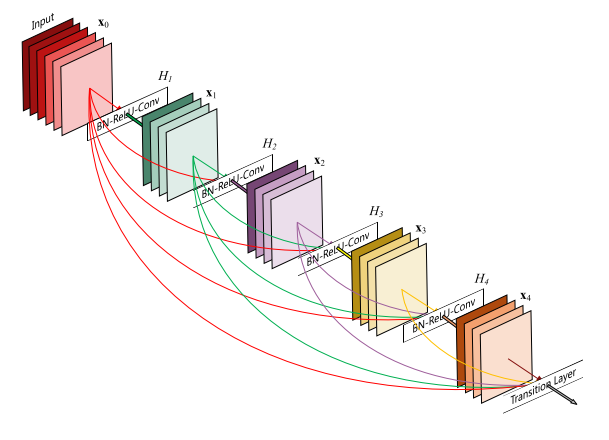
\includegraphics[width=0.5\textwidth]{images/densenet/densenet.png}
\caption{\label{fig:densenet}Densenet structure.}
\end{figure}
\flushbottom
\newpage

\subsection{Best hyper-parameters search spaces}
Hyper-parameters are those parameters whose values are set before the training, unlike other parameters whose values are learned during the training. 
For example learning rate, batch size. \cite{wikihyper}

\subsubsection{Parameters of Densenet}
\begin{itemize}
  \item \textbf{Growth rate}: Number of filters to add per dense block. Growth rate regulates how much information is contributed by each layers to the global state. 
  Global state is the collective knowledge of the network, that is the state of the previous layers are flown into each layer in form of feature-maps, 
  which is considered as global state. Each layer adds k more feature-maps to the current state, when growth rate is k.

  \item \textbf{Nb\_filter}: initial number of filters. -1 indicates initial number of filters will default to 2 * growth\_rate.

  \item \textbf{Nb\_layers\_per\_block}: number of layers in each dense block. Can be a -1, positive integer or a list. If -1, calculates nb\_layer\_per\_block from the network depth. 
  If positive integer, a set number of layers per dense block. If list, nb\_layer is used as provided. Note that list size must be nb\_dense\_block.

  \item \textbf{Depth}: number or layers in the DenseNet.

  \item \textbf{Nb\_dense\_block}: number of dense blocks to add to end.

  \item \textbf{Bottleneck Layers}: To improve computation efficiency a bottleneck layer with 1x1 convolution is introduced before each 3x3 convolution layers. 
  \item \textbf{Compression}: Reduces the feature maps in transition layers and makes the model more compact and computationally efficient.
\end{itemize}



\subsubsection{Other hyper-parameters}
Apart from the densenet there are other general hyper-parameters such as learning rate, batch size for training, optimizer. 


\subsubsection{Grid search strategy}
Since there are lot of parameters, practically, infinite test cases might be designed. To keep the grid search focused and less computationally expensive it makes sense to 
first search for coarser grid of parameters rather than very fine ones. When and if a bracket of parameters are shortlisted which works better than others, the finer parameter
search will be performed only specific to those range of parameters and not the whole grid.

\subsection{Analysis}

\subsubsection{Coarse grid search on Densenet hyper-parameters}
For the estimation of the best performing parameters of Densenet for the branches of the Siamese, first a coarse grid search is been performed with 
\begin{itemize}
 \item Layers per block are chosen among 2,3,4,5,6. For single dense block evaluation goes up-to 12 layers. 
 \item Each network has been evaluated for growth rates of 6,12,18,24,30,36. 
 \item Different dense block sizes of 1,2,3,4.  
 \item Not all the possible combinations has been evaluated as quite extensive as possible
 \item The basic idea here is to narrow down the possible network sizes from the Densenet parameters perspective. There are other parameters but number of dense block, 
 growth rate and layers per block are three main parameters which controls the architecture/size of the network the most.
 \item The parameters compression/reduction and bottleneck are set 0.5 and True respectively because both this parameters controls the compactness of the model and help 
 reducing the parameter required, hence in theory enabling us to evaluate much bigger networks. So the network that is being evaluated here are named Densenet-BC by authors, 
 I.e Densenet with bottleneck and compression.
 \item For more fine grained analysis the compression and bottleneck parameters will also be evaluated. 
 \item nb\_filter values are fixed at 16 for this test
 \item The parameter classes are set to 2, which represents 1 for matching and 0 for not-matching pairs
 \item 96,96 is the input image dimensions. And it’s two channel. So depending on local setting of the keras, “channel-first” or “channel-last” suitable input\_shape is 
 chosen automatically as  2,96,96  or 96,96,2 respectively.
 \item The learning rate used for the test was 2E-4
 \item Dropout for Densenet used as 0.2 to handle over-fitting.  
 \item Epochs are different for different architectures to ensure that the networks are able to train decently %95\% training accuracy. 
 \item From the keras side of the parameters, after concatenating the Densenet branch output feature maps, the “combined features” then passed through a fully-connected  
 layer of 512 filter size, which is followed by Relu activation and Batchnormalization(BN)  and then a dropout(0.5) has been added to ensure better generalization. 
 \item Some of this values needs to be further evaluated as well, how ever current values were obtained using some of manual tuning and assumed to be a decent starting point.
 \item Flatten is used as pooling at the end of the Densenet, it is introduced by this work which replaces the Globalaveragepooling step with a flatten. This causes increase 
 in parameters overall though.
 \item Binary\_crossentropy loss function with sigmoid activation function used for the binary classification, this final layer acts as the binary classifier.
 \item In all the cases the networks are being trained from scratch. The weights = None ensures that no previously trained weights are used.
\end{itemize}

\subsubsection{Coarse grid search parameters summary}
\begin{flushleft} {Fixed hyper-parameters}
\begin{itemize}
 \item Nb\_filter: 16
 \item Subsample initial block: True
 \item Weights : None
 \item Dropout rate : 0.2
 \item Include top : True
 \item Compression : 0.5
 \item Bottleneck : False
 \item Transition pooling : max
\end{itemize}
\end{flushleft}

\begin{flushleft}{Varying Hyper-parameters}
 \begin{itemize}
  \item \textbf{Nb\_layers\_per\_block}:
  \begin{itemize}
   \item \textbf{One dense block architecture (nb\_dense\_block=1):}\\
   '2', '4', '6', '8', '10', '12'
   \item \textbf{Two dense block architecture (nb\_dense\_block=2):}\\
   '2-2', '4-4', '6-6'
   \item \textbf{Three dense block architecture (nb\_dense\_block=3):}\\
   '2-2-2', '4-4-4', '6-6-6'
   \item \textbf{Four dense block architecture (nb\_dense\_block=4):}\\
   '2-2-2-2', '4-4-4-4', '6-6-6-6'
  \end{itemize}
 \item \textbf{Growth rate}:
  \begin{itemize}
  \item Thin layers: 12, 18    
  \item Thick layers: 24, 30    
 \end{itemize}
 \item \textbf{Pooling}:
 \begin{itemize}
  \item Flatten
  \item Average (avg)
 \end{itemize}  
 
\end{itemize}
 
\end{flushleft}

\flushbottom
\newpage

\subsubsection{AUC analysis}
  

\textbf{Conclusion}
\begin{itemize}
 \item It is clear that 4 blocks and 3 blocks network is performing better than the 1 and 2 blocks network
 \item Original paper also used 3 and 4 blocks densenet, so shall we.
\end{itemize}

\subsubsection{Optimal growth rate analysis}
It is also important to find out the best growth rate for each of the architectures(layers per block). For this purpose, the growth rate with mean AUC of test data in 10 trials has been selected,
the Best growth rates across architectures are displayed in the graph below: 


%But it is observed that the architectures with max AUC in 5 evaluations on test data. might consist of different growth rates than the one that displays best mean AUC. For this purpose, histogram of 
%best performing growth rates obtained from mean and max AUC analysis is displayed in the figure below:

%\begin{figure}
%    \centering
%    \begin{subfigure}[b]{0.4\textwidth}
%        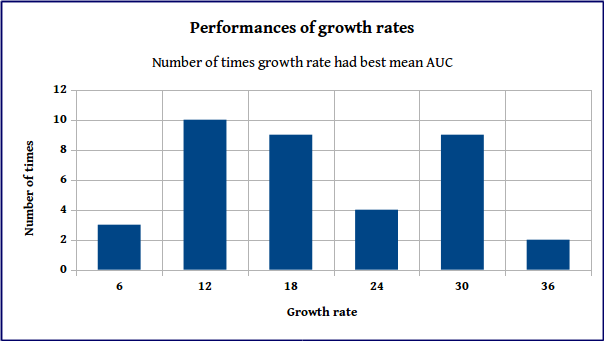
\includegraphics[width=\textwidth]{images/densenet/performances_of_growth_rates_mean_AUC}
%        \caption{Histogram of growth rates depending on mean AUC}
%        \label{fig:mean_auc_histogram}
%    \end{subfigure}
%    ~ %add desired spacing between images, e. g. ~, \quad, \qquad, \hfill etc. 
%      %(or a blank line to force the subfigure onto a new line)
%    \begin{subfigure}[b]{0.4\textwidth}
%        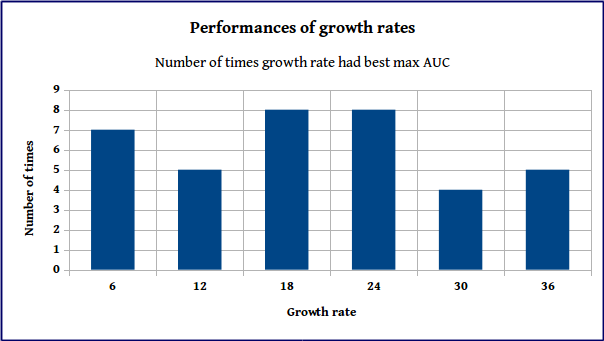
\includegraphics[width=\textwidth]{images/densenet/performances_of_growth_rates_max_AUC}
%        \caption{Histogram of growth rates depending on max AUC}
%       \label{fig:max_auc_histogram}
%    \end{subfigure}    
%    \caption{Cumulative growth rate analysis (histograms)}\label{fig:growthrate_histogram}
%\end{figure}

\textbf{Conclusion}
\begin{itemize}
 \item From the previous study it was concluded that 6,36 growth rates are either too thin or too high so for this test we are not evaluating them.
\end{itemize}

\subsubsection{Total parameters analysis}
\begin{itemize}
 \item How ever as the number of dense blocks keeps getting higher the non-trainable parameters also gets higher. So 4 blocks dense net has most number of non-trainable parameters.
 \item For the comparison 2, 2-2, 2-2-2, 2-2-2-2 blocks parameter sizes are compared below, all recorded for growth rate 18.
 \item FLATTEN VS AVG POOLING and effect
\end{itemize}



\subsubsection{Pooling}


\subsubsection{Standard deviation across blocks}

\subsubsection{Finer grid search analysis}
\begin{itemize}
 \item More detailed analysis for the architectures with different layers per block combination. Specially closer to the highest performing networks.
\end{itemize}

\textbf{Conclusion}

\subsubsection{Nb\_filter analysis}
Initial number of filters. 8,16,32,64 are being evaluated here. Also a comparison between mean AUCs obtained from growth rate 18 and 30 is done under this analysis. Ten evaluations of each test cases has been done.

\textbf{Conclusion}

\subsubsection{Dropout analysis}
Densenet dropout: 10 evaluations each \\


\subsubsection{Bottleneck and Compression(also called reduction) analysis}

\subsubsection{Conclusion}


%\flushbottom
%\newpage

\subsubsection{Batch size analysis}
If the batch size is too low then it takes more time and after a certain size it does not train well too.\\
If the batch size is very big then it may train faster but they generalize lesser as they tend to converge to sharp minimizers of the training function.
TODO add source (https://arxiv.org/abs/1609.04836) 

\textbf{Conclusion}
From the figure 


\subsubsection{Learning rate and optimizer analysis}


\textbf{Conclusion} 

%\begin{center}
% \begin{tabular}{||c c c c c||} 
% \hline\hline
% Learning rate & 0.07 & 0.1 & 0.5 & 1.0 \\ [0.5ex] 
% \hline
% Mean AUC & 0.906 & 0.906 & 0.891 & 0.887 \\ 
% \hline
%\end{tabular}
%end{center}

\subsubsection{Hyper-parameters for final grid search}
%\begin{itemize}
 %\item Layers per block 2-2, 3-4
 %\item nb\_dense\_block 2
 %\item Growth rate 12, 18, 30
 %\item Nb\_filter 16
 %\item Densenet dropout 0.2, 0.4
 %\item Bottleneck False
 %\item Compression 0.3, 0.7
 %\item Learning rate 0.0002 and optimizer Adamax, Learning rate 0.07 optimizer Adadelta, Learning rate 0001 optimizer Nadam
 %item Batch size: 64
 %\item 3 layer network.
%\end{itemize}

\subsubsection{Best results in final grid search(as of now)}


%Divide this into three tables as well for densenet for fc + normal
%\begin{center}
% \begin{tabular}{||c c c c c c c c c c c c c c c c c||} 
% \hline\hline
% Layers & Growth\_rate & dense\_block & nb\_filter & dropout & reduction\_ & bottleneck & fc\_dropout & fc\_filter & Epochs & batch\_size & lr & optimizer & es\_patience & lr\_patience & batch\_size \\ [0.5ex] 
% \hline
% 0.608 & 0.854 & 0.881 & 0.902 & 0.934 & 3 & 0.608 & 0.854 & 0.881 & 0.902 & 0.934 & 3 & 0.608 & 0.854 & 0.881 & 0.902 & 0.934 \\ 
% \hline
% 0.608 & 0.854 & 0.881 & 0.902 & 0.934 & 3 & 0.608 & 0.854 & 0.881 & 0.902 & 0.934 & 3 & 0.608 & 0.854 & 0.881 & 0.902 & 0.934 \\
% \hline
%\end{tabular}
%\end{center}

%\flushbottom
%\newpage

\subsubsection{Intermediate results}
\begin{itemize}
 \item The best results are obtained by the \textbf{Three} blocks network and followed by the \textbf{Four} dense blocks network, while the single and two block network performs worse.(Figures will be added alter). 
 \item While this is generally seen to be in line with the original Densenet theory of bigger and deeper means more better results, this is not the observed behavior in the Densenet Siamese where the two dense block network 
 were performing best. Very interesting.
  \item Right now best result that was obtained is for network [2,2,2] growth rate 30. mean AUC and std (10 trials):  0.946+/-0.008  max:   0.959 %-- Can I make it .95 or .94 ? Prof said leave decimal 3 places
  \item So far the 0.95 AUC results are more frequently obtained in Two channel network, which was the highest in Siamese Densenet network. Even it seems that scoring 0.96 Auc is not rare with the best settings.
 \item In Matias's work it was also found that the simple two channel network better than the siamese network. Using Densenet it is also scene to be the truth.
\end{itemize}

\begin{figure}[ht]
\centering
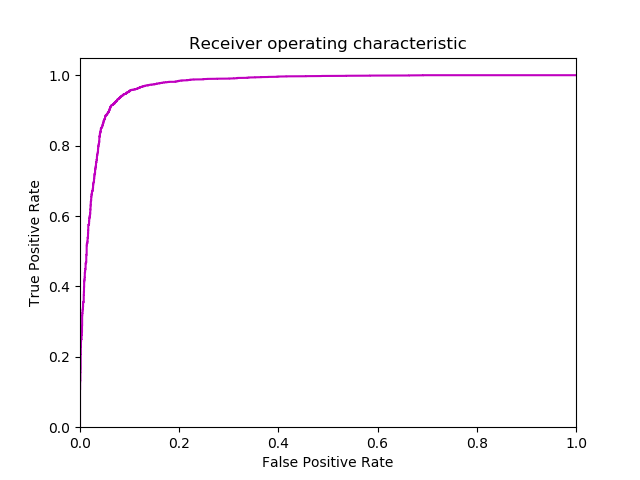
\includegraphics[height= 5cm]{images/densenet/densenet_two_channel_ninetysevenAUC}
\caption{AUC curve Overall best result in both densenet architectures 0.973 AUC (Single run)}
\label{fig:densenet_two_channel_ninetysevenAUC}
\end{figure}

\subsubsection{Conclusion}
\begin{itemize}
 \item State of the art highest AUC \textbf{0.91}
 \item Top result is that of  AUC
 \item Top mean AUC for 10 trials is AUC
\end{itemize}
